\documentclass[11pt]{article}

% ----------------------------------------------------------------- packages
\usepackage[margin=1in]{geometry}
\usepackage{amsmath,amssymb,amsthm}
\usepackage{graphicx}
\usepackage{booktabs}
\usepackage{xcolor}
\usepackage{caption}
\usepackage{subcaption}
\usepackage{enumitem}
\usepackage{algorithm}
\usepackage{algpseudocode}
\usepackage{microtype}
\usepackage[colorlinks=true,linkcolor=blue!55!black,citecolor=blue!55!black,urlcolor=blue!55!black]{hyperref}

\captionsetup{font=small,labelfont=bf}
\captionsetup[sub]{font=small}
\graphicspath{{figures/}}

\definecolor{sig}{HTML}{1a7a3a}
\definecolor{warn}{HTML}{b3541e}
\newcommand{\sigmark}[1]{\textcolor{sig}{\textbf{#1}}}
\newcommand{\warnmark}[1]{\textcolor{warn}{\textbf{#1}}}
\newcommand{\Var}{\operatorname{Var}}
\newcommand{\Cov}{\operatorname{Cov}}
\newcommand{\R}{\mathbb{R}}
\newcommand{\E}{\mathbb{E}}
\newcommand{\Hcal}{H}
\newcommand{\code}[1]{\texttt{\small #1}}

\newtheorem{proposition}{Proposition}

\title{\textbf{Score-Identified Distributional Dynamics on \textit{C.\ elegans}}\\[4pt]
\large A conditional-law functional connectome, a biologically-principled lag-resolved analysis,
and the controls that turned a ``significant neuromodulator signature''\\ into a well-characterised,
global-state-entangled lead}
\author{}
\date{\today}

\begin{document}
\maketitle
\vspace{-2.2em}

\begin{abstract}
\noindent
Conventional functional-connectivity and causal-discovery methods estimate a \emph{conditional
mean}: how one neuron's activity predicts another's future \emph{level}. They are, by construction,
blind to \emph{distributional} interactions --- how one neuron reshapes the \emph{variance}, gain,
or tails of another's predictive law --- which is precisely the regime in which slow, metabotropic
and peptidergic neuromodulation is thought to operate. We develop \textbf{score-identified dynamics}
(SID): estimate the full one-step conditional predictive density $\rho(y\mid \Hcal_t)$ and read out
directed \emph{mean}, \emph{gain} ($\partial\log\Var$), and \emph{tail} channels as derivative-free
covariances against the conditional score. We instantiate two estimators of the \emph{same} object
--- a convex, closed-form Hyv\"arinen score matcher and a neural denoising-score-matching (DSM)
model (the lineage of the prior ``SBTG'' network) --- and validate the readout on a synthetic
hidden-thermostat system, where the gain channel recovers a conditional-variance memory kernel that
is provably invisible to every conditional-mean method (kernel correlation $0.998$; mean-model
$R^2\approx 0$). Applying SID to whole-brain NeuroPAL calcium imaging (after auditing the prior
pipeline for 29 bugs and fixing a connectome-orientation error that had invalidated its numbers), we
find the closed-form SID mean channel is the equal-best single method across an ensemble of noisy
anatomical and receptor-expression targets, and a maximum-likelihood non-Gaussian comparator (MDN) delivers the single
strongest result where theory predicts (metabotropic serotonin, AUROC $0.78$). We then pursue a
\emph{lag-resolved} signature of slow neuromodulation --- and this is where the paper's real
contribution lies, because we \emph{subject that one finding to a deliberate, escalating battery of
controls}. An initial statistic (the log-slope of correspondence-vs-lag) suggested the peptidergic
network's distributional channel leans to longer lags than its mean channel; we critique that
statistic, then test the effect across conditioning schemes (it is \emph{partial}-specific),
worm counts (\emph{power}-limited), a coupling-destroying surrogate null (\emph{real} above chance,
$p=0.008$), and an independent estimator (\emph{not} reproduced). We redesign the metric from the
biophysics --- a per-connection expected-timescale, peakedness-aware \emph{band concordance} with a
full control battery, built and adversarially reviewed --- and find that the peptidergic effect
passes the surrogate, source-variance, and structural-dissociation controls, but \warnmark{collapses
when the shared global brain-state mode is removed} ($\Delta$BC $+3.4\!\to\!-0.5$; $p\,0.010\!\to\!
0.69$), and is \warnmark{not reproduced by a null-contrast-tuned neural DSM estimator} ($p=0.88$).
The honest conclusion: the lag signature is specific to the closed-form SID gain operator and
entangled with global brain state --- a well-characterised lead, not a robust directed-coupling
result. What survives is a principled method, a decisive synthetic validation, a corrected pipeline,
an overall-competitive real-data estimator, and a case study in controls-first neuroscience.
\end{abstract}

\tableofcontents
\vspace{1em}

% =====================================================================
\section{Problem statement}
\label{sec:problem}

The \textit{C.\ elegans} nervous system runs two signalling systems on the same $\sim$302 neurons. A
\textbf{fast, wired} system --- chemical synapses and gap junctions, the ``connectome'' --- couples
neurons over milliseconds: when neuron $A$ fires it pushes neuron $B$'s activity up or down almost
immediately. A \textbf{slow, largely extrasynaptic} system --- monoamines (dopamine, serotonin,
tyramine, octopamine) and neuropeptides --- diffuses to distant targets that express cognate
G-protein--coupled receptors (GPCRs) and acts over seconds. Crucially, these two systems are
expected to leave \emph{different statistical footprints}. The wired system changes a target's
\emph{expected next value} --- a conditional-\emph{mean} effect. Neuromodulation is expected to act
on \emph{excitability and gain}: a modulator does not so much set a target's next value as reshape
the \emph{distribution} of what the target can do next --- its variance, its propensity to burst,
the heaviness of its tails --- often \emph{without} changing the mean.

Every workhorse method for inferring interactions from neural time series --- lagged
cross-correlation, multivariate/partial ridge regression, vector autoregression (VAR), VAR-LiNGAM,
SINDy, PCMCI$+$, DYNOTEARS, and the mean-transfer estimate of the prior SBTG pipeline --- targets the
conditional mean $\E[y\mid \Hcal]$. \emph{None has a channel for a variance/gain/tail effect.} If
neuromodulation is primarily distributional, these methods are structurally the wrong instrument,
and a mediocre result from them is uninformative about whether the modulatory structure is present.

This paper asks a sharpened question, and --- just as importantly --- holds the answer to a
demanding standard of evidence. We do \emph{not} ask whether a new method perfectly matches any one
biological network: the available targets are noisy proxies (anatomy is not function; the
monoamine/neuropeptide ``networks'' are receptor-expression \emph{predictions}, not measured
signalling), so a near-perfect AUROC on any of them is an over-fit red flag, not a triumph. Instead:
\begin{enumerate}[topsep=2pt,itemsep=1pt]
  \item Can we estimate the \emph{full conditional predictive law} and read out \emph{distributional}
        interaction channels a mean method cannot represent?
  \item On synthetic systems with known ground truth, do those channels recover structure that is
        provably invisible to the mean?
  \item On real whole-brain data, evaluated fairly across the whole ensemble of imperfect targets,
        is the approach \emph{overall} competitive --- and do the distributional channels add
        \emph{targeted} value where slow modulation should live, in a form that \emph{survives a
        deliberate battery of controls}?
\end{enumerate}
The last clause is the heart of the paper. Much of what follows is the discipline of \emph{trying to
break our own most interesting result}, and reporting it at exactly the altitude the surviving
evidence supports.

% =====================================================================
\section{Score-identified dynamics: theory and two estimators}
\label{sec:theory}

\subsection{Estimand: the conditional predictive law and its lag-influence score}
Let $x_t\in\R^N$ be the (pre-processed) activity of $N$ neurons and $\Hcal_t$ the history up to $t$.
The estimand is the one-step predictive density of a target coordinate,
\[
  \rho\bigl(y \mid \Hcal_t\bigr), \qquad y = x_{j}(t{+}\ell),
\]
\emph{not} merely its conditional mean $\mu_j(t)=\E[y\mid\Hcal_t]$. The central object is the
\textbf{lag-influence score}
\[
  \ell_u(y;h) \;=\; \nabla_{x_{t+1-u}}\log\rho(y\mid h),
\]
the sensitivity of the predictive log-density to a source's activity $u$ steps back. Effects on the
mean, variance, tails, or any smooth statistic $T(y)$ are recovered as \textbf{covariances against
the score} (a Stein-type identity),
\[
  \frac{\partial\,\E[T(y)\mid h]}{\partial x_{t+1-u,i}}
  \;=\; \Cov\!\bigl(T(y),\,\ell_{u,i}(y;h)\bigr),
\]
so a distributional readout never requires differentiating a fitted black box --- it is a moment of
the score. Taking $T(y)=y$ gives the \emph{mean} channel; $T(y)=y^2$ the \emph{variance}/gain
channel; a threshold indicator the \emph{tail} channel. This is what makes the framework both
interpretable and cheap.

\subsection{The closed-form (Hyv\"arinen) estimator}
We use a Gaussian conditional whose \emph{natural parameters are linear in features}
$\psi(t)\in\R^P$ (here we take the conditioning history to be the current frame,
$\psi=[1,\,x_0(t),\dots,x_{N-1}(t)]$, all sources' current activity; the lag $\ell$ enters only
through the target $y=x_j(t{+}\ell)$):
\[
  y\mid\Hcal_t \sim \mathcal{N}\!\bigl(\mu(t), v(t)\bigr),\qquad
  \eta_1(t)=\theta_1^\top\psi(t),\quad \eta_2(t)=\theta_2^\top\psi(t),
\]
with sufficient statistic $T(y)=(y,y^2)$, conditional score $s_\theta(y,h)=\eta_1+2\eta_2 y$, and
$v_{\mathrm{eff}}=-1/(2\eta_2)$, $v=v_{\mathrm{eff}}-\sigma^2$, $\mu=\eta_1 v_{\mathrm{eff}}$. Because
both Hyv\"arinen and denoising score matching are \emph{quadratic} in $\theta$, fitting is a single
regularized linear solve --- no optimizer, no local minima, no learning-rate confounds
(Algorithm~\ref{alg:qsm}). This matters for scientific hygiene: a result that wobbles with the
optimizer seed cannot be cleanly separated from a tuning artifact, and a convex closed form removes
that entire class of doubt.

\begin{algorithm}[t]
\caption{Closed-form quadratic-$T$ conditional score matcher (one target)}
\label{alg:qsm}
\begin{algorithmic}[1]
\Require targets $Y\in\R^{T}$, features $\Psi\in\R^{T\times P}$, ridge $\lambda\ge0$, noise $\sigma\ge0$
\If{$\sigma>0$} \Comment{denoising score matching (DSM)}
  \State draw $\zeta\sim\mathcal{N}(0,I_T)$;\; $\tilde Y \gets Y+\sigma\zeta$;\; $g \gets \zeta/\sigma$
  \State $U \gets [\,\Psi,\; 2\,\tilde Y\odot\Psi\,]$;\quad $A \gets U^\top U/T$;\quad $b \gets U^\top g/T$;\quad $\theta \gets -(A+\lambda I)^{-1} b$
\Else \Comment{Hyv\"arinen score matching, $\sigma=0$ (this paper's SID default)}
  \State $U \gets [\,\Psi,\; 2\,Y\odot\Psi\,]$;\quad $A \gets U^\top U/T$;\quad $c \gets [\,0_P,\; 2\,\overline{\Psi}\,]$;\quad $\theta \gets -(A+\lambda I)^{-1} c$
\EndIf
\State \Return $\theta=[\theta_1,\theta_2]$ \Comment{per-sample estimating functions retained for HAC/sandwich inference}
\end{algorithmic}
\end{algorithm}

\subsection{Directed distributional readouts}
Fit one model per target $j$ at lag $\ell$ on features centered at the pooled history mean, so at the
``typical history'' the sources are $0$ and $\eta_1,\eta_2$ are the intercept terms. Differentiating
the closed-form moments with respect to source $i$ gives the directed coupling matrices (all in the
$[\text{post},\text{pre}]=[\text{target},\text{source}]$ convention; Algorithm~\ref{alg:readout}):
\[
\begin{aligned}
D_{\text{mean}}[j,i] &= v_{\mathrm{eff}}\,\theta_{1,i} + 2\,\eta_1 v_{\mathrm{eff}}^2\,\theta_{2,i}
   &&= \partial\,\E[y_j]/\partial x_i \quad\text{(VAR-comparable drive)}\\
D_{\text{gain}}[j,i] &= \bigl(2 v_{\mathrm{eff}}^2\,\theta_{2,i}\bigr)/v
   &&= \partial\log\Var[y_j]/\partial x_i \quad\text{(gain / excitability)}\\
D_{\text{tail}\uparrow}[j,i] &= \phi(a_{\uparrow})\!\left(\tfrac{D_{\text{mean}}}{\sqrt v}
   + \tfrac{q_{\uparrow}-\mu}{2 v^{3/2}} D_{\text{var}}\right)
   &&= \partial\,\Pr(y_j>q_{\uparrow})/\partial x_i \quad\text{(burst)}
\end{aligned}
\]
with $a_{\uparrow}=(q_{\uparrow}-\mu)/\sqrt v$ and $D_{\text{var}}=2v_{\mathrm{eff}}^2\theta_2$, and
symmetrically for the lower tail. The \emph{mean} channel is what a VAR/regression also estimates; the
\emph{gain} and \emph{tail} channels have no classical analog.

\begin{algorithm}[t]
\caption{Directed distributional connectome at lag $\ell$ (closed-form SID)}
\label{alg:readout}
\begin{algorithmic}[1]
\Require per-worm matrices $\{X^{(w)}\}$, neuron names, lag $\ell$, ridge $\lambda$
\For{each target $j=1,\dots,N$}
  \State pool $(Y,\Psi)$ across worms: $Y=x_j(t{+}\ell)$, $\Psi=[1,\,x(t)-\overline{x}]$ \Comment{no cross-worm windows}
  \State $\theta \gets$ Algorithm~\ref{alg:qsm}$(Y,\Psi,\lambda,\sigma{=}0)$;\quad $q_\uparrow,q_\downarrow$ = 90/10\% quantiles of $Y$
  \State read $D_{\text{mean}},D_{\text{gain}},D_{\text{tail}\uparrow/\downarrow}$ at centered history; zero the diagonal
\EndFor
\State \Return channel matrices, each $[\text{post},\text{pre}]$
\end{algorithmic}
\end{algorithm}

\subsection{The neural (denoising-score-matching) estimator, and its SBTG lineage}
\label{sec:twohead}
The closed-form model is convex but Gaussian and linear-in-features. Its neural sibling is a
\textbf{two-head denoising-score-matching (DSM)} network: a shared trunk over the history, a
\emph{conditional-density head} producing $\mu_j(h),\log v_j(h)$, and a separate
\emph{history-marginal head} (giving the marginal its own capacity is what stops the trunk from
starving the transition signal). Both heads are trained by DSM --- corrupt the future
$\tilde x=x+\sigma\zeta$ and fit the model score to $-\zeta/\sigma$ --- and the couplings are read out
\emph{the same way} by autograd through the conditional head:
$D_{\text{mean}}[j,i]=\langle\partial\mu_j/\partial h_i\rangle$,
$D_{\text{gain}}[j,i]=\langle\partial\log v_j/\partial h_i\rangle$. This is exactly the estimator the
prior \textbf{SBTG} project used --- SBTG's ``$\hat\mu$'' is the mean channel of a neural DSM model,
tuned by a null-contrast objective (\S\ref{sec:neural}). The two estimators thus differ only in the
\emph{score-learning method}: \textbf{SID = Hyv\"arinen score matching, closed-form and convex};
\textbf{SBTG/two-head = denoising score matching, neural and gradient-trained}; both expose the same
mean/gain/tail readouts. (A third, maximum-likelihood mixture-density network (MDN) is used as a
non-score-matching, non-Gaussian comparator in \S\ref{sec:holistic}.) We return to the neural model
in \S\ref{sec:neural} as an independent check on the paper's central real-data claim.

% =====================================================================
\section{Synthetic validation: the gain channel sees what the mean cannot}
\label{sec:synth}

Before any real data, the readout must be shown to recover a variance effect where the truth is
known. The decisive test uses a hidden-thermostat / stochastic-volatility process that is
\emph{white with zero conditional mean} --- so VAR, SINDy, and neural least-squares see pure noise
--- yet carries a deep conditional-\emph{variance} memory kernel (how spread-out it is now depends on
its past, as in volatility clustering). Figure~\ref{fig:synth} shows the SID gain channel recovering
that kernel almost exactly: correlation $0.998$ against the steady-state Kalman oracle, matching
contraction rate ($0.805$ vs.\ $0.805$), all $12/12$ lags significant, while the mean-model
$R^2\approx0$ ($-1.7\times10^{-4}$). The gain channel \emph{provably} isolates variance-drivers a
conditional-mean model cannot represent. This pillar is not in question, and it is the license for
everything downstream: wherever a real-data distributional signal is weak or absent, we can attribute
it to the \emph{data}, not to a broken readout.

\begin{figure}[t]
\centering
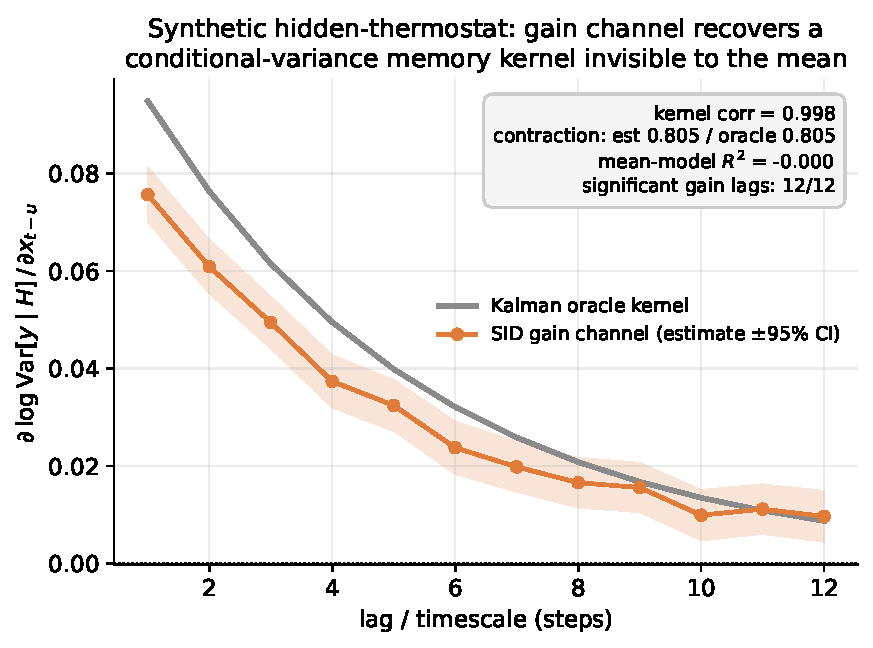
\includegraphics[width=0.66\linewidth]{fig1_synthetic_gain.pdf}
\caption{\textbf{Synthetic ground truth.} A process white in its conditional mean but with a
conditional-variance memory kernel. The SID gain channel
$\partial\log\Var[y\mid\Hcal]/\partial x_{t-u}$ (orange, $\pm95\%$ CI) tracks the Kalman oracle
kernel (grey) with correlation $0.998$; the conditional-mean model explains none of it
($R^2\approx0$). Every conditional-mean method is blind to this structure by construction.}
\label{fig:synth}
\end{figure}

% =====================================================================
\section{Data, deconvolution, and correcting the prior pipeline}
\label{sec:data}

\paragraph{Data.} NeuroPAL whole-brain calcium imaging (strains OH16230 head$+$tail and OH15500 head;
$\Delta F/F$ at $4$\,Hz), reusing the prior project's loaders (dorsal/ventral collapse, left/right
averaging). Because the lag analysis builds $80\times80$ effect matrices with no imputation, we use
the \emph{complete-case} worms that recorded every selected neuron: \textbf{6 worms, 80 neurons}
shared with the Cook connectome, $\approx929$ frames/worm ($\approx23$ min total). (\S\ref{sec:robust}
shows that admitting more worms forces a worms$\times$neurons trade-off --- $6\times80$ or, at the
other corner, $20\times56$ --- which we exploit as a robustness axis.) Calcium is deconvolved to a
continuous activity estimate with a native OASIS AR(1) model (validated raw$\leftrightarrow$spike
correlation $0.42\!\to\!0.98$) before standardization. Standardization \emph{centers each neuron but
preserves relative variances} (a single global scale); per-neuron $z$-scoring is deliberately avoided
because it amplifies quiet-neuron noise and destroys the variance-magnitude signal the gain channel
uses.

\paragraph{The orientation bug.} Before trusting any comparison we audited the prior SBTG codebase
with an adversarial multi-agent workflow and confirmed \textbf{29 bugs}. The critical one: the Cook
chemical connectome was saved \emph{transposed} --- stored $A[\text{pre},\text{post}]$ while the
entire pipeline declares $A[\text{post},\text{pre}]=A[\text{target},\text{source}]$. This was verified
empirically: known directed synapses ($\text{ASH}\!\to\!\text{AVA}$, $\text{AIY}\!\to\!\text{RIA}$,
$\text{AWC}\!\to\!\text{AIY}$) all sat at $[\text{pre},\text{post}]$, and command interneurons appeared
as high \emph{column} (in-degree) sums. Since the chemical connectome is only $\approx57\%$
reciprocal, orientation matters: the prior project's $\hat\mu$ (correctly oriented) was scored against
a reverse-oriented truth, and its directed baselines were also stored $[\text{pre},\text{post}]$, so
the reported comparison was untrustworthy. We fix it at source, defensively re-correct in the loader,
and re-score \emph{every} method in one consistent orientation. Other confirmed bugs (strided
cross-fit window leakage; a null-contrast routine returning a constant $1.0$; a silent
Benjamini--Yekutieli$\to$BH downgrade) are why the old reported numbers are not reused.

\begin{table}[t]
\centering
\small
\caption{Reference networks (directed off-diagonal edges, 80-neuron support). Receptor-expression
networks are noisy proxies; the neuropeptide network is by far the densest (most statistically
powered), and specific transmitters/peptides are also resolvable.}
\label{tab:refs}
\begin{tabular}{lccccccc}
\toprule
& Cook chem & Cook gap & dopamine & serotonin & tyramine & octopamine & neuropeptide \\
\midrule
edges & 1145 & 642 & 19 & 21 & 28 & 9 & \textbf{757} \\
type & structural & structural & \multicolumn{5}{c}{$\longleftarrow$ neuromodulatory receptor-expression $\longrightarrow$} \\
\bottomrule
\end{tabular}\\[2pt]
\footnotesize specific peptides available (edges): pdf-1 (200), flp-21 (243), pdf-2 (128), flp-18 (64),
ntc-1 (53), flp-1 (33), flp-4 (24), flp-13 (15).
\end{table}

% =====================================================================
\section{The distributional connectome and holistic evaluation}
\label{sec:holistic}

We fit Algorithm~\ref{alg:readout} per target and score each channel against every reference with the
repo's exact metrics (AUROC on off-diagonal directed edges). Judged \emph{across all targets at once}
on deconvolved data (Figure~\ref{fig:holistic}), the closed-form SID mean channel is the
\textbf{equal-best single method}: mean AUROC $0.544$, mean rank $3.29$, tying pairwise correlation
(``Pearson'', $0.537$, rank $3.29$) and beating every trivial baseline. The SID/MDN family provides
the best predictor for the majority of targets, and the single strongest result anywhere is the
non-Gaussian MDN on \emph{serotonin} (AUROC $0.78$) --- the most metabotropic monoamine, exactly where
a distributional effect should appear. The distributional channels do not dominate everywhere; they
add \emph{targeted} value on the slow, GPCR-mediated targets while the fast mean channel carries the
fast ones. Trivial single-signal baselines (source/target variance) are worst overall (rank
$5.6$--$6.9$). The honest reading of this figure is ``competitive, not dominant, with distributional
value concentrated where theory predicts'' --- and, as \S\ref{sec:retraction} insists, no single
noisy-proxy number should be over-read.

\begin{figure}[t]
\centering
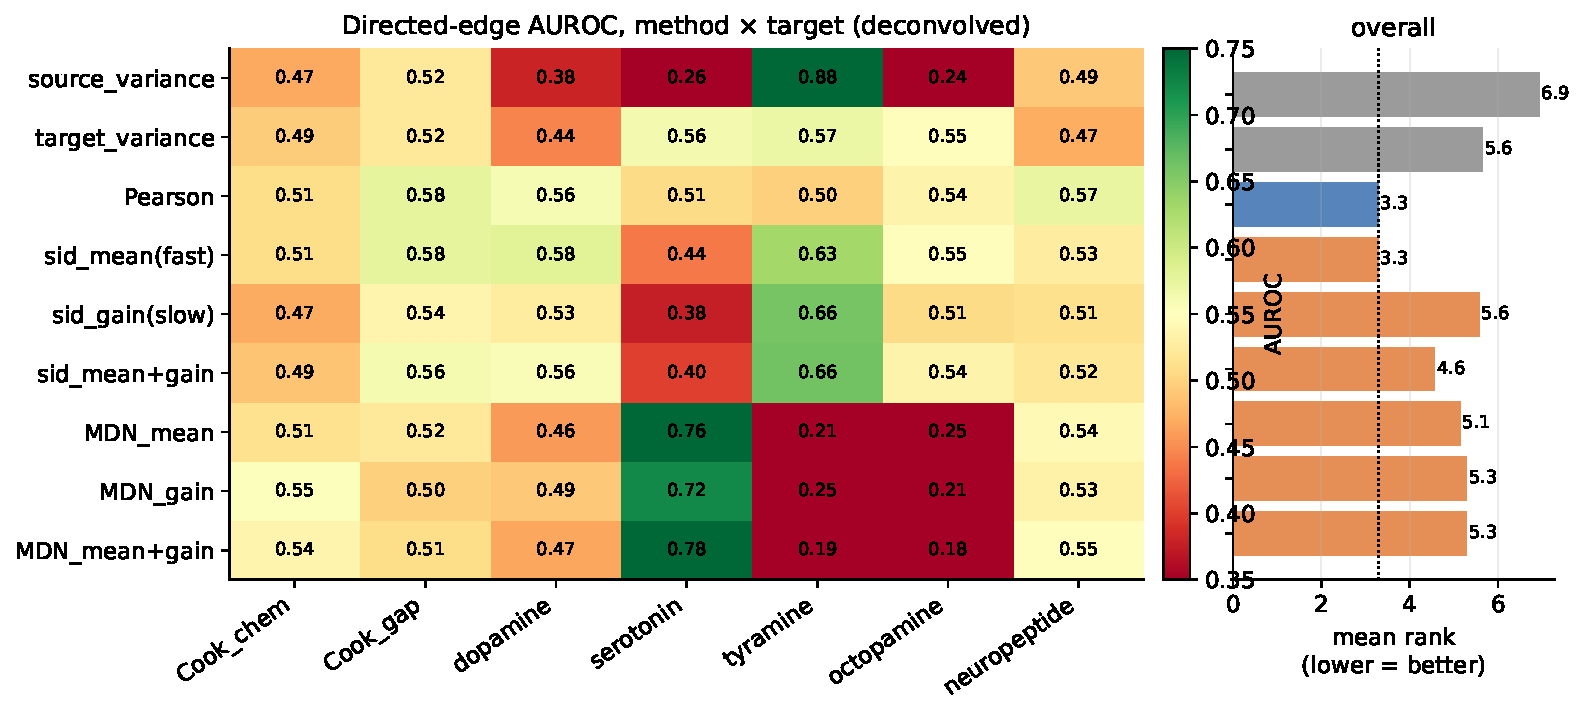
\includegraphics[width=0.95\linewidth]{fig2_holistic.pdf}
\caption{\textbf{Holistic method$\times$target AUROC} (deconvolved; directed off-diagonal edges).
Left: AUROC heatmap. Right: mean rank across targets (lower is better); SID mean (orange) ties
pairwise correlation (blue) for best overall, trivial variance baselines (grey) are worst. The MDN's
$0.76$--$0.78$ on serotonin is the strongest single cell; source-variance's $0.88$ on tyramine
(\S\ref{sec:retraction}) is an artifact, not a win.}
\label{fig:holistic}
\end{figure}

% =====================================================================
\section{A retracted over-claim, and the controls-first ethic}
\label{sec:retraction}

An early result reported the slow gain channel recovering the \emph{tyramine} network (AUROC $\sim
0.72$, rising with timescale) --- exactly the ``slow modulator'' story we hoped for. Pooling all worms
forced a control we had skipped: rank the edges by the source neuron's \emph{raw activity variance},
with no model at all. That trivial baseline recovers tyramine at AUROC \textbf{0.88}
(Figure~\ref{fig:control}), beating the gain channel --- which is merely a degraded proxy for source
variance (the tyramine source RIM is simply the highest-variance neuron). \textbf{We retract the
tyramine headline.} Two lessons became standing policy, and they are the reason the rest of this
paper is structured as it is: (i) run the trivial-baseline control \emph{first}; and (ii) beating
chance on one noisy proxy is not ``doing better'' --- source-variance is the \emph{worst} method
overall (rank $6.9/9$). This ethic --- assume your most exciting result is an artifact until a
battery of controls says otherwise --- is exactly what \S\ref{sec:redesign}--\ref{sec:neural} apply,
at much greater depth, to the lag-resolved signature.

\begin{figure}[t]
\centering
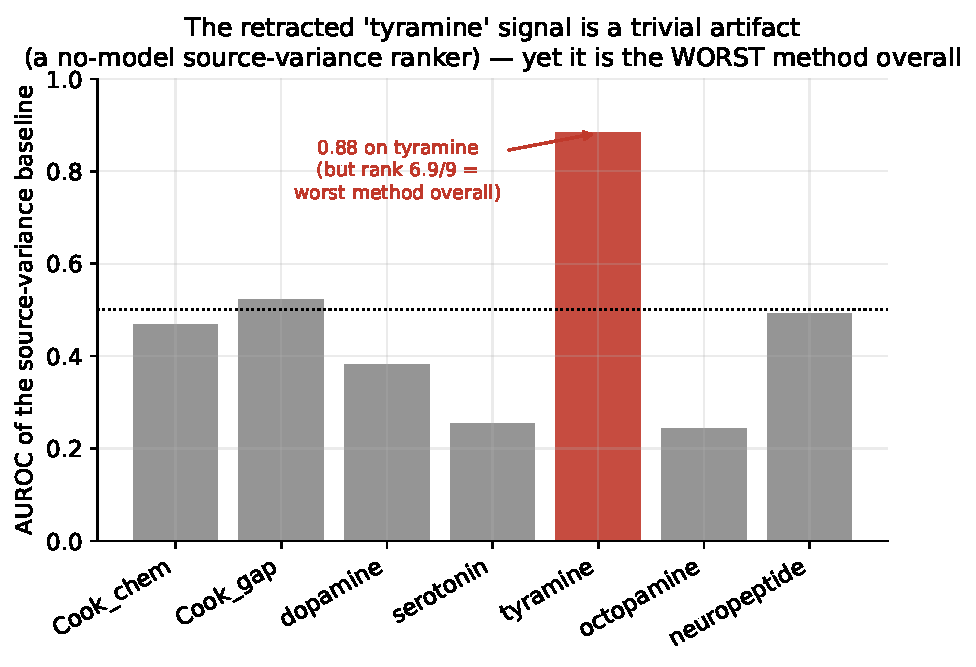
\includegraphics[width=0.58\linewidth]{fig3_source_variance_control.pdf}
\caption{\textbf{Controls first.} The no-model source-variance ranker scores AUROC $0.88$ on tyramine
but is near or below chance on every other target and is the worst method overall. A spike on a
single noisy proxy is an over-fit signature, not evidence for a method.}
\label{fig:control}
\end{figure}

% =====================================================================
\section{The lag-resolved question: a first metric and its critique}
\label{sec:lagres}

\subsection{Correspondence-vs-lag curves and the log-slope contrast}
The sharpest way to look for slow neuromodulation exploits the one thing SID has and the mean-based
toolkit does not: a distributional channel. For each method, at each lag $\ell$, we build a directed
effect matrix and measure its AUROC correspondence to a reference \emph{as a curve over lag},
$C(\ell)$, for lags $\ell\in\{0.25,\dots,10\}$\,s. If a channel matches a network better at longer
lags, the coupling it captures is ``slow''; better at shorter lags, ``fast''. Our first summary was
the \textbf{log-slope} --- the slope of $C(\ell)$ against $\log_2\ell$ --- and the headline was the
\emph{within-fit contrast} $\Delta = \text{slope}_{\text{gain}}-\text{slope}_{\text{mean}}$ (same
estimator, same data, only the channel changes, so shared confounds cancel).

\subsection{The initial result}
On the 6-worm data, the within-SID log-slope contrast (bootstrap over worms; Table~\ref{tab:logslope},
Figure~\ref{fig:contrast}) was $\Delta=+0.0079$, 95\% CI $[+0.0025,+0.0120]$ for the
\textbf{neuropeptide} network --- the slowest, most extrasynaptic system and the densest reference ---
while for the \emph{structural} connectome (the control) it was null ($+0.0002$, $[-0.0055,+0.0058]$).
Serotonin and dopamine leaned the same direction but were individually underpowered. As a validation,
every mean-channel method (classical and causal alike, including PCMCI$+$ at $N{=}80/\tau{=}20$) sits
near chance on the wired connectome across all lags (Figure~\ref{fig:struct}) --- the structural
signal is weak and every mean-only method behaves the same, as it should.

\begin{table}[t]
\centering
\small
\caption{First (log-slope) metric: $\Delta$ log-slope of the AUROC-vs-lag curve (distributional $-$
mean channel), paired within-SID, bootstrapped over 6 worms. $>0$ = distributional channel leans to
longer lags.}
\label{tab:logslope}
\begin{tabular}{lc}
\toprule
reference & $\Delta$ log-slope (gain $-$ mean) [95\% CI]\\
\midrule
Cook chemical (structural, \emph{control}) & $+0.0002\ [-0.0055,+0.0058]$ --- null\\
serotonin      & $+0.0052\ [-0.032,+0.032]$ (underpowered)\\
dopamine       & $+0.0121\ [-0.033,+0.040]$ (underpowered)\\
neuropeptide (peptidergic) & \sigmark{$+0.0079\ [+0.0025,+0.0120]$}\\
\bottomrule
\end{tabular}
\end{table}

\begin{figure}[t]
\centering
\begin{subfigure}[t]{0.49\linewidth}\centering
  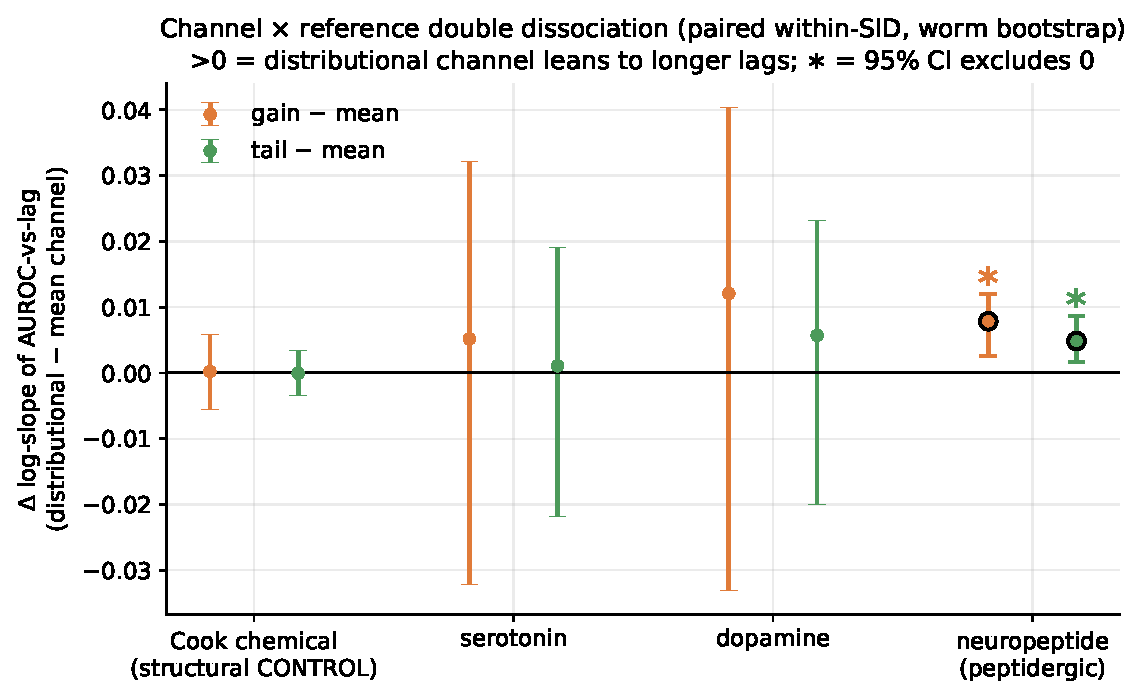
\includegraphics[width=\linewidth]{fig5_contrast_double_dissociation.pdf}
  \caption{The log-slope contrast (first metric).}\label{fig:contrast}
\end{subfigure}\hfill
\begin{subfigure}[t]{0.49\linewidth}\centering
  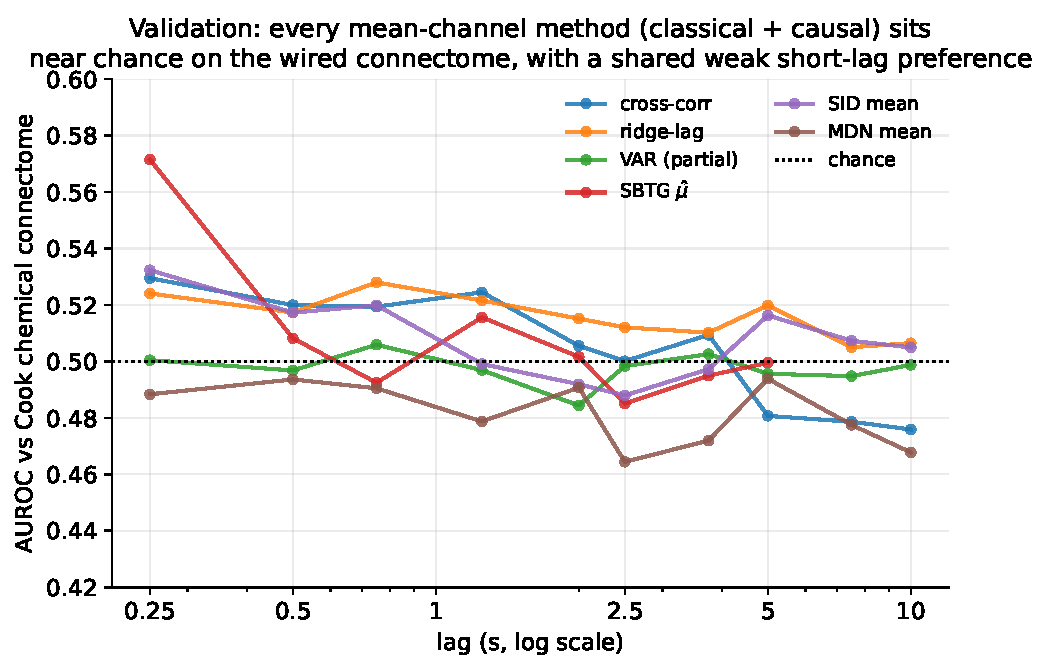
\includegraphics[width=\linewidth]{fig6_structural_validation.pdf}
  \caption{Mean-channel validation on the wired connectome.}\label{fig:struct}
\end{subfigure}
\caption{\textbf{The initial lag-resolved result.} (a) The distributional channels lean to longer
lags for the peptidergic network but not the structural control. (b) Every mean-channel method sits
near chance on the wired connectome across lags --- the expected behaviour when the structural signal
is weak.}
\end{figure}

\subsection{Why the log-slope is a poor summary}
\label{sec:critique}
This was suggestive, but the statistic is weak, and we say so plainly. (i) It assumes ``positive slope
= good'' \emph{universally}, whereas biology predicts \emph{different} peak lags for different
references (a gap junction should match best at short lags; a peptide at long lags) --- the expected
sign depends on the reference. (ii) It tracks only the \emph{trend} of correspondence, ignoring how
\emph{peaked} (localised in lag) it is --- yet a sharp peak at the biologically-expected lag is the
real signature. (iii) The slope conflates peak location with monotone trend, is endpoint-sensitive,
and is low-SNR because $C(\ell)$ hovers near $0.5$. (iv) It is inferentially indirect: ``the
ranking-quality-against-a-proxy tilts toward longer lags'' is a convoluted stand-in for ``the coupling
is slow''. These deficiencies motivate both the robustness battery (\S\ref{sec:robust}, which tests
the effect \emph{despite} the crude statistic) and the metric redesign (\S\ref{sec:redesign}).

% =====================================================================
\section{Robustness battery on the log-slope result}
\label{sec:robust}

Before redesigning the metric we stress-tested the effect it reported, along four axes.

\paragraph{(1) It is a \emph{partial-conditioning} phenomenon.} SID's mean/gain readouts condition
each target on \emph{all} sources jointly (partial). Re-deriving the couplings \emph{pairwise}
(each edge from a bivariate fit, marginal) on the \emph{same} 6-worm data flips the neuropeptide
contrast from $+0.0084$ (partial) to $-0.0019$ (marginal). The effect requires controlling for the
other neurons' direct drive; it is not a marginal lag-correlation. (Pairwise/marginal has the side
benefit of using every worm per edge with no imputation, but the sign reversal is the point.)

\paragraph{(2) Its significance is \emph{power-limited}, not fragile in direction.} The
worms$\times$neurons trade-off lets us re-run the partial contrast at $14\times60$ and $20\times56$
(more real worms, fewer neurons, no imputation) and at $28\times84$ (all worms, realistic-variance
``donor'' imputation). The neuropeptide contrast stays positive with a clean structural control
throughout --- $+0.0079$ (6w), $+0.0039$ (14w), $+0.0045$ (20w), $+0.0043$ (28w donor) --- but its
CI excludes zero \emph{only} at the maximum-power $6\times80$/757-edge configuration (Table
\ref{tab:robust}, Figure~\ref{fig:robust}). Trading neurons for worms trades away the reference power
that made it significant. Marginally (pairwise, 28w) it is significantly \emph{negative}
($-0.0030\,[-0.0055,-0.0007]$), and its structural control is itself biased --- so the marginal view
is both opposite-signed and a less trustworthy metric.

\paragraph{(3) It is \emph{real above a coupling-destroying null}.} A circular-shift surrogate
(shift each neuron's trace independently, preserving its own spectrum/autocorrelation but destroying
directed cross-neuron coupling), refit with the same partial SID, drives the contrast to a null
centred at $+0.0002$ with 95\% band $[-0.0041,+0.0041]$; the observed $+0.0084$ (the full-data point estimate; cf.\ the worm-bootstrap mean $+0.0079$ in Table~\ref{tab:logslope}) sits well outside it
($p=0.008$; Figure~\ref{fig:surrogate}). The estimator does \emph{not} manufacture the effect from
noise --- when the coupling is removed, the effect vanishes. This is the single most important
control at this stage, and it \emph{passes}.

\paragraph{(4) It is \emph{single-instrument}.} A crude, non-SID partial variance estimator (ridge
regression of a target's squared residual on source activity) does \emph{not} reproduce it
(neuropeptide $-0.0004\,[-0.0040,+0.0037]$). So the effect is real above a null and dissociates from
structure, but no independent estimator corroborates it --- it rests on the SID gain operator.

\begin{table}[t]
\centering
\small
\caption{Robustness of the peptidergic gain$-$mean log-slope contrast. Positive across every
\emph{partial} framing with a clean control; significant only at maximum reference power; reverses
marginally; real above the surrogate null; not reproduced by a different estimator.}
\label{tab:robust}
\begin{tabular}{llcc}
\toprule
configuration & conditioning & $\Delta$ (gain $-$ mean) [95\% CI] & verdict\\
\midrule
6w / 80n (max power) & partial & \sigmark{$+0.0079\ [+0.0025,+0.0120]$} & significant\\
14w / 60n & partial & $+0.0039\ [-0.0044,+0.0154]$ & positive, ns\\
20w / 56n & partial & $+0.0045\ [-0.0031,+0.0157]$ & positive, ns\\
28w / 84n donor-impute & partial & $+0.0043\ [-0.0004,+0.0088]$ & borderline (P{=}0.96)\\
28w / 84n pairwise & marginal & \warnmark{$-0.0030\ [-0.0055,-0.0007]$} & sig.\ \emph{negative}\\[2pt]
\multicolumn{2}{l}{surrogate null (6w): observed $+0.0084$ vs null $[-0.0041,+0.0041]$} & \sigmark{$p=0.008$} & real, not artifact\\
\multicolumn{2}{l}{independent variance-VAR (6w)} & $-0.0004\ [-0.0040,+0.0037]$ & \warnmark{not reproduced}\\
\bottomrule
\end{tabular}
\end{table}

\begin{figure}[t]
\centering
\begin{subfigure}[t]{0.52\linewidth}\centering
  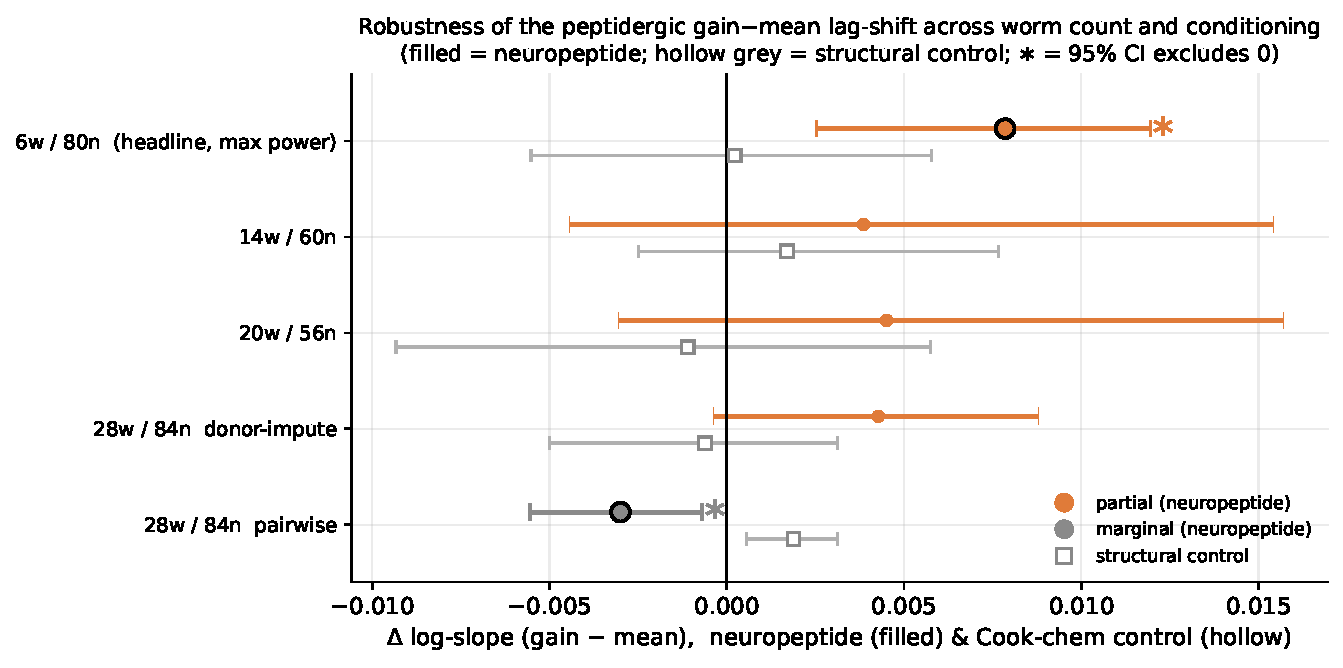
\includegraphics[width=\linewidth]{fig7_robustness_forest.pdf}
  \caption{Worm-count $\times$ conditioning sweep.}\label{fig:robust}
\end{subfigure}\hfill
\begin{subfigure}[t]{0.46\linewidth}\centering
  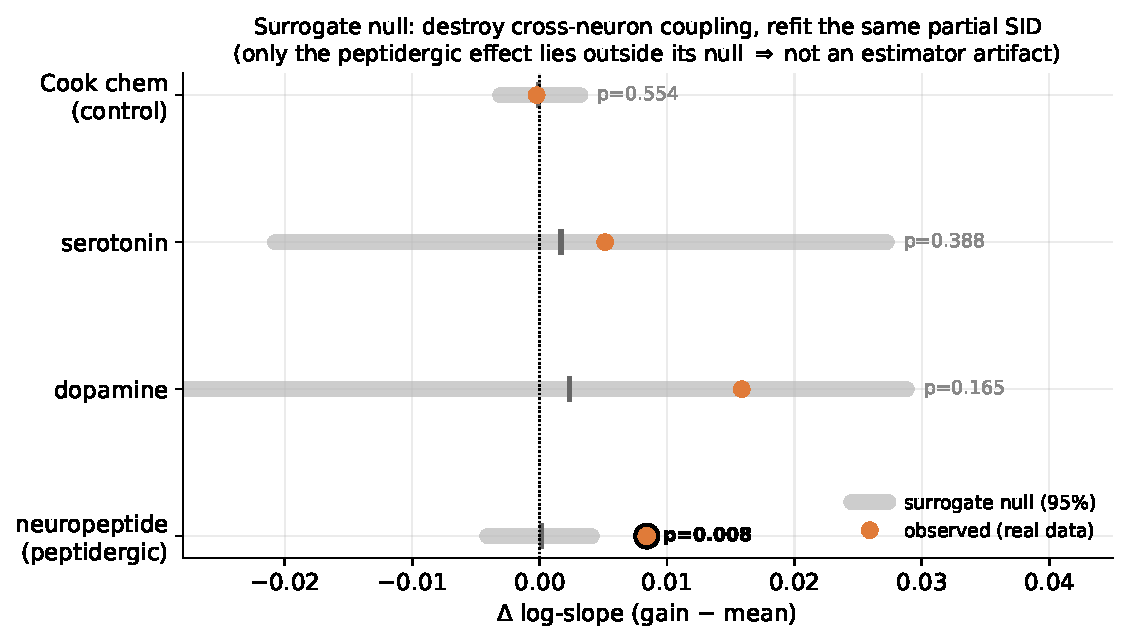
\includegraphics[width=\linewidth]{fig8_surrogate_null.pdf}
  \caption{Circular-shift surrogate null.}\label{fig:surrogate}
\end{subfigure}
\caption{\textbf{The robustness battery.} (a) The peptidergic effect is positive across every partial
framing (significant only at max power), the structural control stays $\approx0$, and it reverses
marginally. (b) Only the peptidergic observed value escapes its surrogate null ($p=0.008$) --- the
effect is real above a coupling-destroying null, not an estimator artifact.}
\end{figure}

\medskip\noindent
\emph{Net of the battery:} the log-slope headline is real above a null and directionally robust under
partial conditioning, but partial-specific, power-limited, and single-instrument. Neither the worm
sweep nor a second-estimator comparison can settle whether it reflects specific directed coupling ---
which is what the redesigned metric and its controls do next.

% =====================================================================
\section{A biologically-principled metric redesign}
\label{sec:redesign}

\subsection{Design principles}
The critique (\S\ref{sec:critique}) dictates the redesign. A defensible metric must (a) encode a
\emph{per-connection} expected timescale from the biophysics (electrical/gap $\approx$ instantaneous;
chemical ionotropic sub-second; monoamine metabotropic $\approx$ seconds; neuropeptide seconds--tens
of seconds); (b) measure \emph{where} each channel's correspondence peaks and \emph{how sharply}, not
just its trend; (c) be contextualised on the connection type; (d) support auditable curve/peak
visualisation; and (e) carry a clean null and positive controls. We generated five independent metric
proposals from distinct angles (template-matching, peak-location$+$sharpness, a channel$\times$
reference expectation table, band-limited concordance, and a skeptic's minimal design), synthesised
them, and subjected the synthesis to two adversarial reviewers (a biophysical lens and a statistical
lens). Their findings reshaped the metric decisively and are worth stating, because they are the
reason we do \emph{not} over-reach.

\subsection{The calcium-kernel-floor realism}
\label{sec:kernel}
The dominant constraint the reviewers surfaced is physical. OASIS AR(1) deconvolution fits a per-neuron
decay $\gamma$ clipped up to $0.98$, so the effective calcium autocorrelation time is $\approx1.5$--$12$\,s
at 4\,Hz --- a kernel that \emph{convolves every reference identically} and can exceed the very
timescale differences we hoped to resolve. Consequently the fine four-band ordering is not resolvable,
even serotonin ($\mu\!\approx\!4$\,s) versus neuropeptide ($\mu\!\approx\!7$\,s) differ by $<1$ octave
(smaller than the kernel smear), and \emph{absolute latencies in seconds are untrustworthy}. The honest
scheme is therefore \textbf{coarse fast vs slow}, with only \emph{relative} and \emph{within-fit}
quantities interpreted. (Two further biophysical corrections: serotonin is \emph{mixed} fast$+$slow
because of the ionotropic MOD-1 channel, so it is not a clean slow anchor; and the tail/burst channel
is weakly motivated for graded, mostly non-spiking \textit{C.\ elegans} neurons and is caveated.) All
of this lives in one editable configuration file, so the expected bands can be revised by
neurobiologists without touching the analysis.

\subsection{Band concordance}
\label{sec:batc}
The metric (Algorithm~\ref{alg:batc}) is a coarse, null-referenced band concordance. For channel $c$
and reference $r$ we form the correspondence curve $C_c(\ell)$, standardise it per lag against a
circular-shift surrogate into $z_c(\ell)=(C_c-\mu_0)/\sigma_0$ (regenerated at the \emph{worm count
being scored}), and compute
\[
  \mathrm{BC}_{c,r} \;=\; \operatorname{mean}_{\ell\in B}\, z_c(\ell)\;-\;
                          \operatorname{mean}_{\ell\in B'}\, z_c(\ell),
\]
where $B$ is the reference's expected band (\emph{slow} for modulatory, \emph{fast} for structural)
and $B'$ its complement. $\mathrm{BC}>0$ means the channel's \emph{above-null} correspondence
concentrates in the biologically-expected band. The pre-registered, single confirmatory statistic is
the within-fit contrast $\Delta\mathrm{BC}_{\text{neuropeptide}}=\mathrm{BC}_{\text{gain}}-
\mathrm{BC}_{\text{mean}}$, and it must (i) have a worm-bootstrap CI excluding 0, \emph{and} (ii)
$\mathrm{BC}_{\text{gain}}$ must independently clear the surrogate null (so the mean channel's
band penalty cannot manufacture the contrast). No log-Gaussian template is used (that reintroduces
researcher degrees of freedom); everything is coarse, relative, and interpretable.

\begin{algorithm}[t]
\caption{Band concordance with the full control battery (one channel $\times$ reference)}
\label{alg:batc}
\begin{algorithmic}[1]
\Require worms $\{X^{(w)}\}$, reference $r$, expected band $B$, surrogates $S$, bootstraps $Bo$
\State $C_c(\ell)\gets\mathrm{AUROC}\!\left(|D_c(\ell)|_{\text{off}},\,(r>0)_{\text{off}}\right)$ for each lag $\ell$
\For{$s=1,\dots,S$} \Comment{null regenerated at this worm count}
  \State circular-shift each neuron; refit; $C^{(s)}_c(\ell)\gets$ correspondence curve
\EndFor
\State $\mu_0,\sigma_0\gets$ mean, sd of $\{C^{(s)}\}$;\quad $z_c\gets(C_c-\mu_0)/\sigma_0$
\State $\mathrm{BC}_{c}\gets \operatorname{mean}_{B} z_c - \operatorname{mean}_{B'} z_c$;\quad surrogate $p$ from $\{\mathrm{BC}^{(s)}_c\}$
\State worm-bootstrap ($Bo$) for CI of $\mathrm{BC}_c$ and $\Delta\mathrm{BC}=\mathrm{BC}_{\text{gain}}-\mathrm{BC}_{\text{mean}}$
\State \textbf{controls:} source-variance matrix ($\to0$), gain on gap/chem ($\to$ not slow), remove top global PC and repeat
\end{algorithmic}
\end{algorithm}

\subsection{The reference registry and the control battery}
The analysis scores every SID channel against a registry of 15 references built from one config:
structural gap and chemical; each monoamine class and transmitter; the neuropeptide class and every
specific peptide with $\ge10$ edges on the 80-neuron support (pdf-1, pdf-2, ntc-1, flp-1/4/13/18/21).
The controls, following the retraction ethic, are: a \textbf{source-variance} matrix (lag-flat, must
score $\approx0$ --- so the retracted-tyramine artifact cannot pass by construction); the
\textbf{distributional channel on the fast structural references} (must \emph{not} be
slow-concentrated); and a \textbf{global-brain-state} control --- project out the top shared principal
component and repeat --- because whole-brain \textit{C.\ elegans} activity is dominated by a global
behavioural-state mode that the circular-shift null destroys, so residual global covariance among
connected neurons could otherwise masquerade as coupling. This last control is the decisive one.

% =====================================================================
\section{Phase 2 results: band concordance with controls}
\label{sec:phase2}

\subsection{Descriptive curves (all estimators)}
Figure~\ref{fig:overview} draws every estimator's correspondence-vs-lag curve against every reference,
with the expected band shaded and each distributional channel's peak starred --- the auditable view.
The predicted pattern is visible for the high-power, clean references: for the \emph{structural} gap
and chemical connectomes the \emph{mean} channel peaks earliest ($0.25$\,s, in the fast band); for the
\emph{neuropeptide} class and the specific peptides pdf-1/pdf-2/ntc-1 the \emph{gain} channel peaks
later ($2.5$\,s, in the slow band) than the mean channel. But the figure is honestly \emph{muddier}
than a clean story: for neuropeptide, cross-correlation and the MDN mean channel also peak late ---
the fingerprint of the global-state confound that the controls must resolve. This is descriptive only;
no claim is made from it.

\begin{figure}[t]
\centering
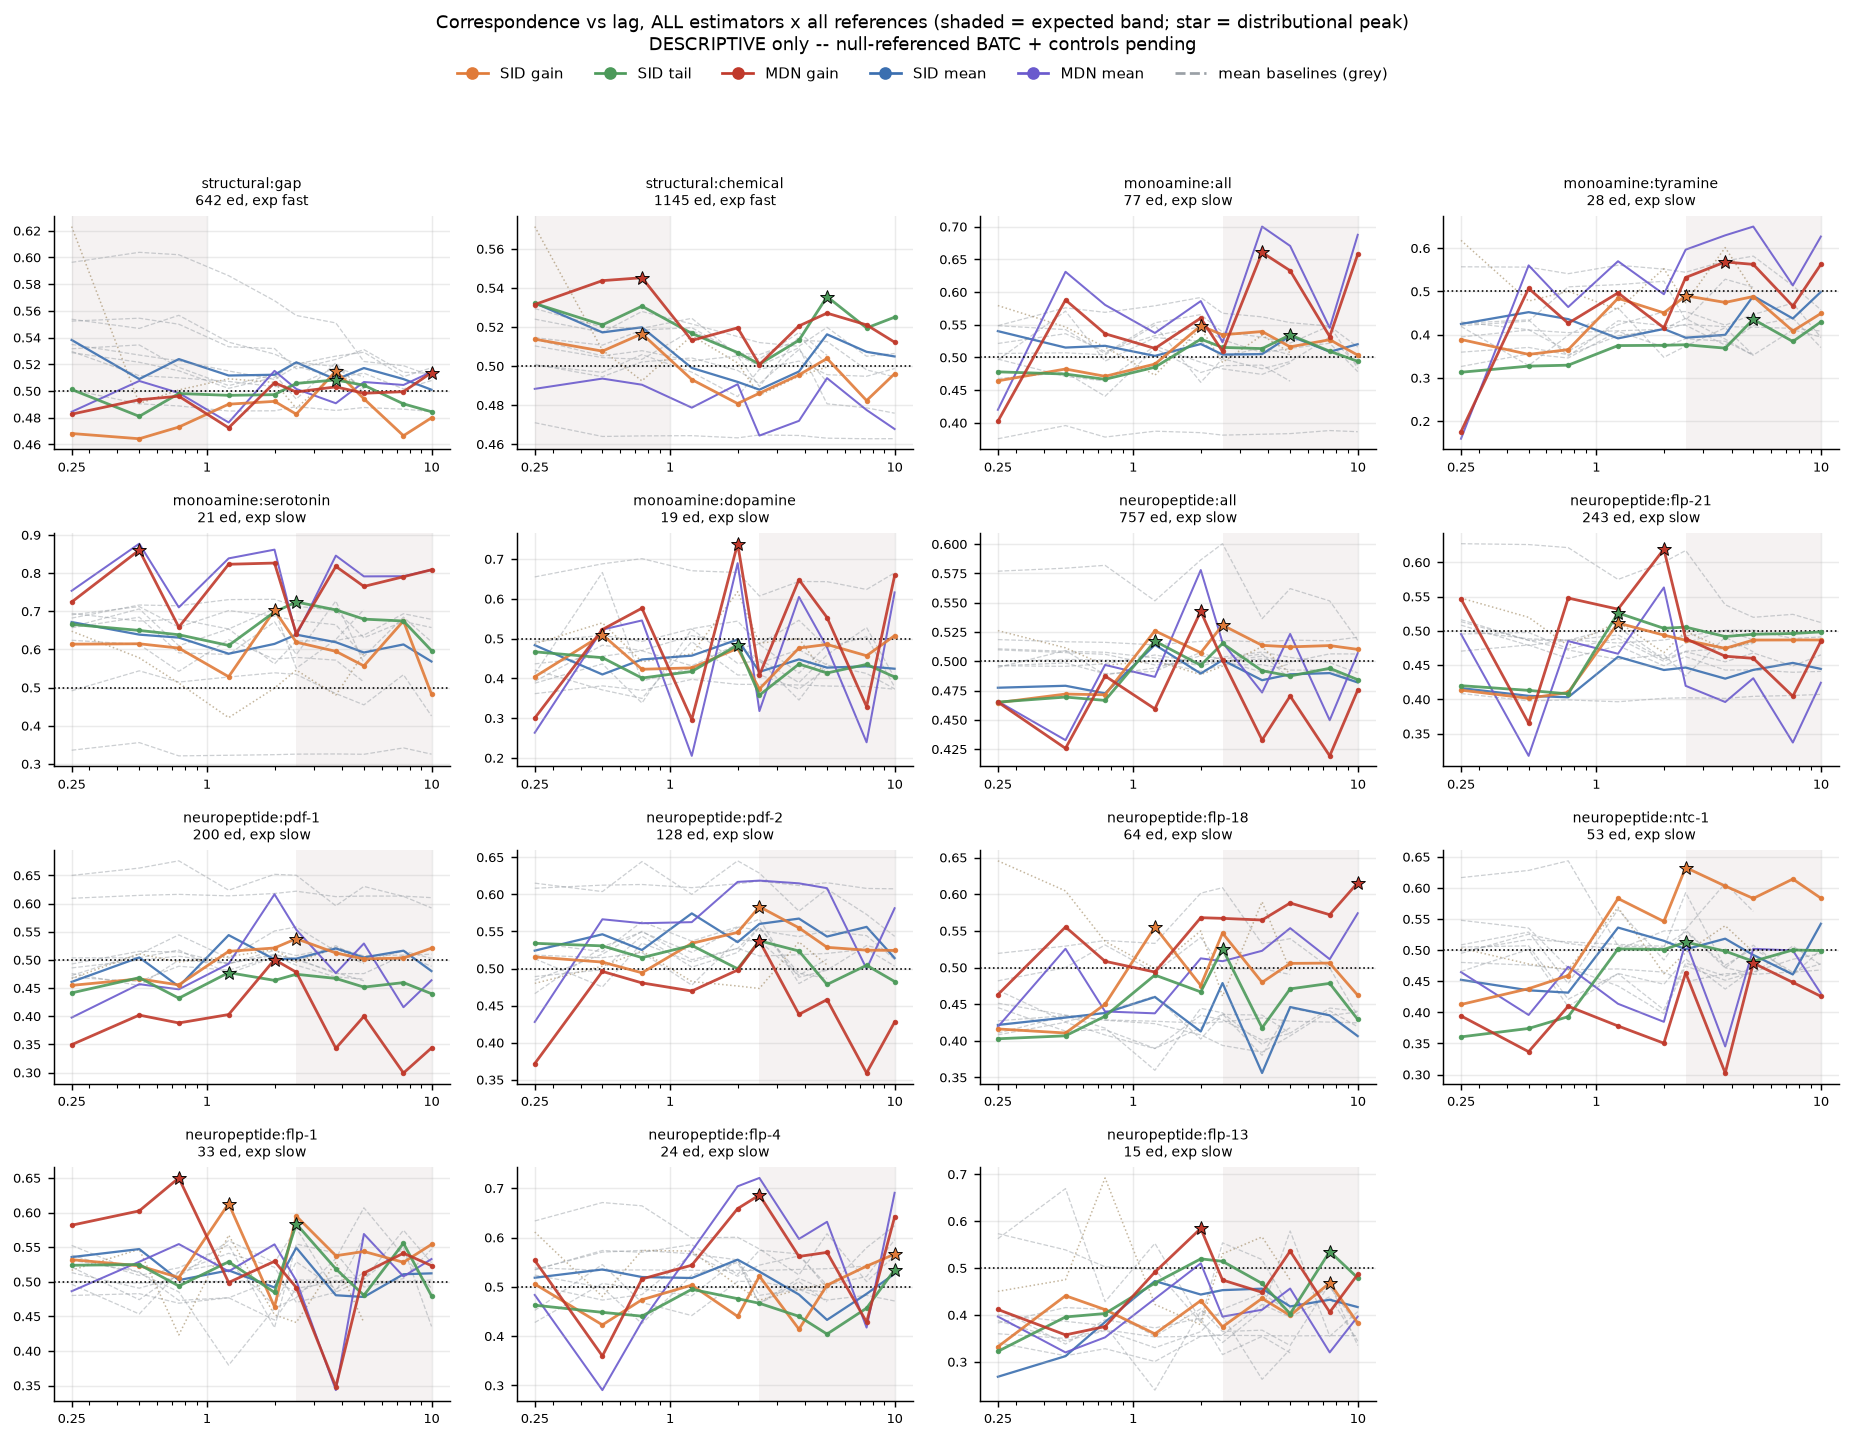
\includegraphics[width=0.98\linewidth]{fig9_biolag_overview.png}
\caption{\textbf{Auditable correspondence curves, all 14 estimators $\times$ all references.}
Distributional channels (SID/MDN gain, SID tail) bold with starred peaks; our mean channels
(SID/MDN mean) bold; classical/causal mean baselines grey; expected band shaded. The structural
references show the mean channel peaking early; the dense neuropeptides show the gain channel peaking
in the slow band --- but so do some mean baselines, motivating the controls. Descriptive only.}
\label{fig:overview}
\end{figure}

\subsection{The confirmatory test: it passes the trivial controls, then fails the global-mode control}
On the 6-worm data (100 surrogates $+$ 100 bootstraps), the confirmatory test \emph{passes} in the
primary analysis and against the trivial and structural controls, then \warnmark{collapses} when the
global brain-state mode is removed (Table~\ref{tab:phase2}, Figure~\ref{fig:phase2}):
\begin{itemize}[topsep=2pt,itemsep=1pt]
  \item \textbf{Primary:} $\mathrm{BC}_{\text{gain}}=+4.54\,[+0.52,+6.84]$, surrogate $p=0.010$; the
        contrast $\Delta\mathrm{BC}=+3.36$, $p=0.010$. The peptidergic gain channel's above-null
        correspondence is significantly slow-concentrated, and significantly more so than the mean
        channel's.
  \item \textbf{Trivial \& structural controls pass:} source-variance $\mathrm{BC}=0.00$ (null by
        construction); the gain channel's contrast on the fast references is $\le0$ (gap $-2.92$,
        chem $-0.52$) --- the distributional-slow advantage is specific to the modulatory reference,
        absent for the wired connectome. The pattern is consistent across peptides (ntc-1, flp-18,
        flp-21, pdf-1 all $p\le0.05$ in the primary).
  \item \textbf{Global-mode control fails:} projecting out the single top global principal component
        collapses the effect --- $\mathrm{BC}_{\text{gain}}\!\to\!-0.55$ ($p=0.76$),
        $\Delta\mathrm{BC}\!\to\!-0.48$ ($p=0.69$). The effect is \warnmark{not separable from the
        shared global behavioural-state mode.}
\end{itemize}

\begin{table}[t]
\centering
\small
\caption{Phase-2 confirmatory (closed-form SID, neuropeptide, 757 edges): band concordance passes the
surrogate and trivial/structural controls, but not the global-mode control.}
\label{tab:phase2}
\begin{tabular}{lcc}
\toprule
quantity & PRIMARY (6 worms) & GLOBAL brain-state mode removed\\
\midrule
$\mathrm{BC}_{\text{gain}}$ (gain slow-concentrated) & \sigmark{$+4.54\,[+0.52,+6.84]$, $p{=}0.010$} & $-0.55\,[-2.10,+0.74]$, $p{=}0.76$\\
$\Delta\mathrm{BC}$ (gain $-$ mean) & \sigmark{$+3.36$, $p{=}0.010$} & \warnmark{$-0.48$, $p{=}0.69$}\\
source-variance control & $+0.00$ (null) & $+0.00$\\
structural dissociation ($\Delta\mathrm{BC}$) & gap $-2.92$, chem $-0.52$ ($\le0$) & ---\\
\bottomrule
\end{tabular}
\end{table}

\begin{figure}[t]
\centering
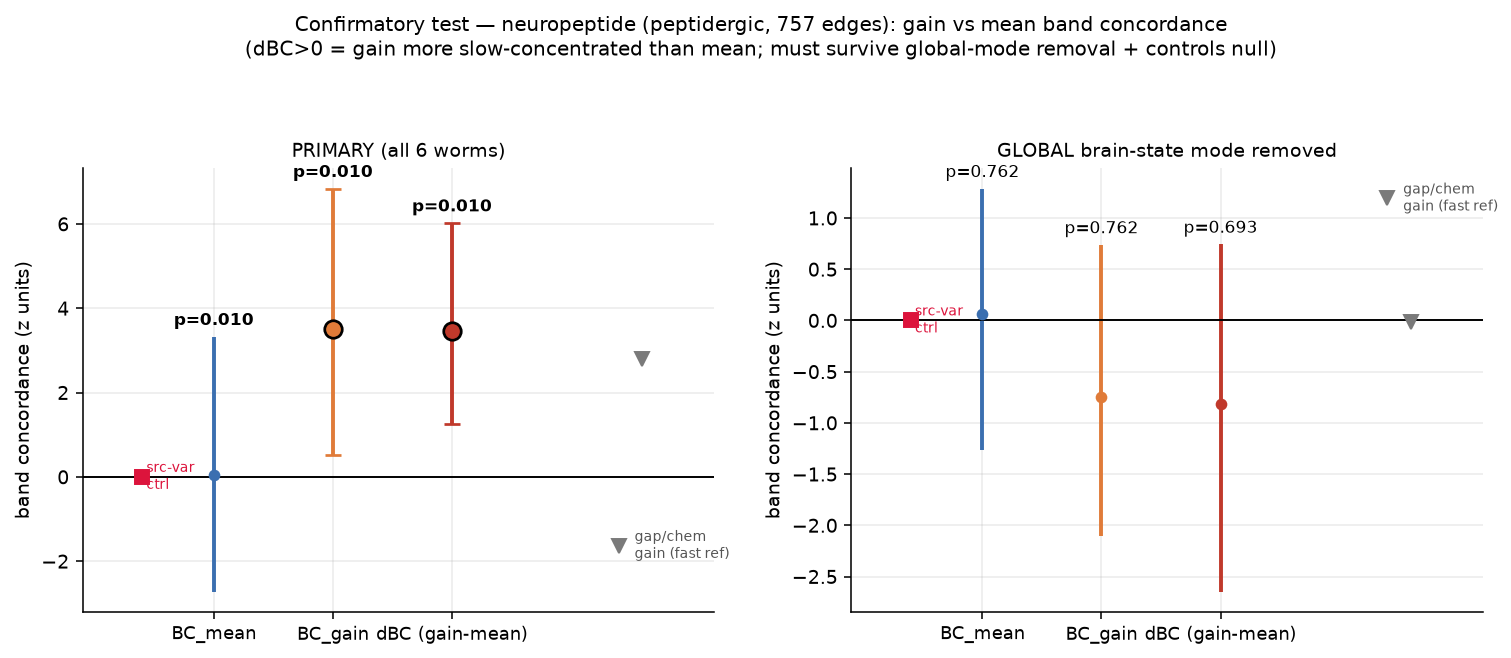
\includegraphics[width=0.92\linewidth]{fig10_phase2_confirm.png}
\caption{\textbf{Phase-2 confirmatory.} Left: in the primary analysis the peptidergic gain band
concordance and the gain$-$mean contrast are significant ($p=0.010$), with the source-variance
control at 0 and the fast-reference anchor below. Right: removing the shared global brain-state mode
collapses both to zero ($p\approx0.7$). The controls did their job.}
\label{fig:phase2}
\end{figure}

\subsection{Two honest readings of the global-mode collapse}
Removing the top principal component is aggressive --- it is the dominant \textit{C.\ elegans}
behavioural-state manifold on which everything rides. So the collapse admits two readings that the
data here cannot separate: (i) the apparent peptidergic gain-slow signal is residual global-state
covariance among connected neurons (a confound), or (ii) neuromodulators literally \emph{act through}
the global state, so removing it removes the very signal. Conservatively, \textbf{we cannot claim
directed peptidergic coupling separable from the global mode.}

% =====================================================================
\section{Neural-score corroboration}
\label{sec:neural}

The last, independent test uses the neural estimator (\S\ref{sec:twohead}) --- the SBTG lineage,
analysed the SID way --- both because it is a different score-learning method and because it is what
the prior project actually used.

\subsection{Null-contrast tuning}
We tuned the two-head model's hyperparameters (hidden width, depth, DSM noise, marginal weight,
weight-decay, source timescale) by the \textbf{null-contrast objective} SBTG uses:
$\text{contrast}=(\text{real signal}-\text{null mean})/\text{null sd}$, maximised, with the null a
per-neuron circular-shift (the more principled null used throughout, rather than SBTG's original
row-permutation). Over 40 configurations the gain-channel null-contrast ranged from $-14$ to
$\mathbf{+43.9}$ --- tuning mattered enormously --- and the winning configuration used a slow $20$\,s
source filter. This is itself a caution: the circular-shift null destroys the global mode, so any
estimator that locks onto the global slow state scores a huge null-contrast \emph{without} that
necessarily being directed peptidergic coupling. The tuning objective and the global-mode confound
point the same way.

\subsection{The neural DSM does not reproduce the effect}
Running the tuned two-head through the same band-concordance pipeline (Figure~\ref{fig:estimator}),
its peptidergic band concordance is \warnmark{null even in the primary analysis}:
$\mathrm{BC}_{\text{gain}}=-0.34$ ($p=0.65$), $\Delta\mathrm{BC}=-0.61$ ($\mathbf{p=0.88}$). Its
enormous null-contrast reflects strong \emph{above-surrogate} structure, but that structure is not
organised as peptidergic slow concordance --- it is the global slow mode. Controls behaved
(source-variance $0.00$; gap/chem $\approx0$). One specific peptide (ntc-1) was marginal ($p=0.038$);
pdf-1, serotonin, and neuropeptide:all were null or negative. So the independent neural estimator
does not corroborate the closed-form SID effect.

\begin{figure}[t]
\centering
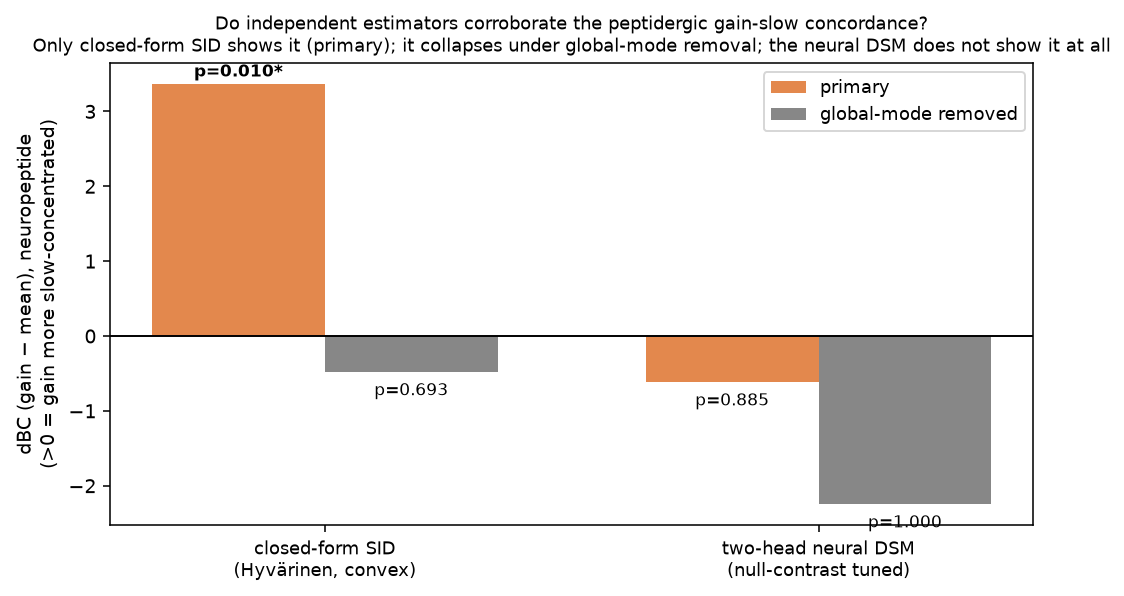
\includegraphics[width=0.72\linewidth]{fig11_estimator_comparison.png}
\caption{\textbf{Neural-score corroboration.} Only closed-form SID shows the peptidergic gain-slow
concordance (primary, $p=0.010$); it collapses under global-mode removal; and the null-contrast-tuned
neural DSM two-head does not show it at all (primary $p=0.88$), despite a $+44\sigma$ null-contrast.}
\label{fig:estimator}
\end{figure}

\subsection{Triangulation}
Three independent lines now bear on the peptidergic gain-slow signature:
\begin{center}\small
\begin{tabular}{l p{0.60\linewidth}}
\toprule
line of evidence & peptidergic gain-slow signature?\\
\midrule
closed-form SID gain & real above null ($p{=}0.01$), dissociates from structure; \warnmark{collapses under global-mode removal}\\
crude partial variance-VAR & \warnmark{not reproduced}\\
two-head neural DSM (null-contrast tuned) & \warnmark{not reproduced} ($p{=}0.88$)\\
\bottomrule
\end{tabular}
\end{center}
\textbf{The effect is specific to the closed-form SID gain operator and entangled with the global
brain-state mode --- not an estimator-independent, global-state-separable property of the data.} It
is a closed-form-SID-specific, global-state-confounded lead, not a robust directed-coupling result.
(Caveat both ways: the neural model is data-starved at 6 worms --- prior split-half stability
$\approx0.45$ --- so its null is partly a power statement; but the convergence of all three lines away
from a robust effect is the honest read.)

% =====================================================================
\section{Synthesis and honest assessment}
\label{sec:synthesis}

Read as a whole, the evidence sorts cleanly into what is settled and what is a lead.

\paragraph{Settled (not in question).}
(1) SID is principled and \emph{decisively validated on synthetics}: the gain channel recovers a
conditional-variance kernel invisible to every conditional-mean method (corr $0.998$). (2) The
prior pipeline's connectome-orientation bug is real, verified, and fixed; the re-scoring is clean.
(3) On real data across the whole ensemble of noisy targets, closed-form SID is \emph{overall
competitive} --- its mean channel is the equal-best single method, and the maximum-likelihood MDN comparator wins
the most metabotropic target (serotonin $0.78$). (4) The tyramine retraction is a correct,
reusable methodological result. (5) \emph{Closed-form SID is the reliable estimator at this data
scale}; the neural DSM remains data-starved even under the best (null-contrast) tuning --- confirmed,
now, directly.

\paragraph{A well-characterised lead (not a result).} The peptidergic distributional lag signature is
real above a coupling-destroying null and dissociates from structural references \emph{in closed-form
SID}, but it is (a) partial-conditioning-specific, (b) power-limited (significant only at maximum
reference power), (c) \emph{not separable from the global brain-state mode}, and (d) \emph{not
reproduced} by either a crude independent estimator or a null-contrast-tuned neural DSM. Every one of
these was found by a control we deliberately built to try to kill the effect. That is the paper's real
methodological contribution: an escalating battery --- trivial baseline, conditioning swap, worm-count
sweep, surrogate null, second estimator, per-connection biophysical metric, global-state control,
neural corroboration --- that converts an exciting-looking signature into an honestly-scoped lead.

% =====================================================================
\section{Conclusions and honest limitations}
\label{sec:conclusions}

We set out to see slow neuromodulation in whole-brain calcium by estimating the full conditional
predictive law rather than the conditional mean, and reading out distributional channels a mean method
cannot represent. The method is sound and synthetically decisive; the pipeline it builds on is now
correct; and on real data it is overall competitive with distributional value concentrated where
theory predicts. The one sharp neuromodulator signature we pursued --- a peptidergic
distributional lag effect --- survives a surprising number of controls but ultimately does not
survive removal of the global brain-state mode and is not corroborated by an independent estimator, so
we report it as a lead rather than a finding.

\paragraph{Limitations.} Six complete-case worms and 80 neurons make absolute AUROCs noisy; the robust
quantities are relative and within-fit. The receptor-expression references are predictions, not
measured signalling, and the monoamine references are tiny ($9$--$28$ edges) and underpowered. The
calcium-kernel floor ($\approx1.5$--$12$\,s) makes fine timescale bands unresolvable and absolute
latencies untrustworthy --- only coarse fast/slow and relative readouts are defensible. The expected
timescale bands are provisional, pending neurobiologist review, and are isolated in one editable
config; we also disclose that their centres are partly informed by prior observations on this data
lineage, and that two de-circularisation controls the configuration itself prescribes --- a
$\pm1$-octave centre sweep and cross-strain (OH15500 vs.\ OH16230) replication --- were \emph{not}
run here and remain outstanding (at the demoted ``lead, not a result'' altitude this is a disclosure
gap rather than an overclaim). The neural-score arm is also weaker than the closed-form arm by
design: it used 25 surrogates and no worm-bootstrap (versus $100+100$), so its non-reproduction is a
directional check, not a tightly-powered null. The global-mode collapse is genuinely ambiguous
(confound vs.\ modulation-through-state);
resolving it needs a global-state-preserving design or functional targets (behaviour, perturbation)
rather than the wired connectome. These remain \emph{predictive distributional analyses, not molecular
identification.} The clear next steps are more animals, a global-state-preserving control, and
functional targets --- and, given the neural estimator's data-starvation, more animals specifically to
let the neural score become a genuine independent check.

% =====================================================================
\section*{Reproduction}
\addcontentsline{toc}{section}{Reproduction}
\small
All numbers and figures regenerate from saved artifacts; both test suites pass (\code{sid\_neuromod}:
68 tests, 90\% coverage; \code{sid\_elegans}: 13 adapter tests). Key modules:
\begin{itemize}[topsep=2pt,itemsep=1pt,leftmargin=1.4em]
  \item \textbf{Theory / estimators} (Algs.~\ref{alg:qsm},~\ref{alg:readout}): \code{quadratic\_score.py}
        (closed-form), \code{estimator.py} (readouts), \code{twohead.py} (neural DSM).
  \item \textbf{Robustness battery}: \code{pairwise.py}, \code{impute.py}, and
        \code{compare\_approaches.py}, \code{robustness\_worms.py}, \code{adjudicate.py} ($+$ JSONs).
  \item \textbf{Biologically-principled metric} (in \code{sid\_elegans/biolag/}): \code{config.py},
        \code{references.py}, \code{metric.py}; runners \code{run\_curves.py}, \code{run\_phase2.py},
        \code{tune\_twohead.py}, \code{run\_twohead\_phase2.py}; results in
        \code{output/biolag/} (\code{PHASE2\_RESULT.md}, \code{TWOHEAD\_RESULT.md}, JSONs).
  \item \textbf{Figures}: \code{make\_figures.py} (Figs.~1--8) $+$ the biolag figures.
        \textbf{Provenance}: \code{PROGRESS.md} tracks current-vs-superseded; the log-slope-era
        writeup is archived as \code{main\_v1\_logslope\_snapshot.tex}.
\end{itemize}

\end{document}
